\documentclass[11pt,a4paper]{article}
\usepackage{a4wide}
\usepackage{enumerate}
\usepackage{enumitem}
\usepackage{pcptex}
\usepackage{xspace}

\begin{document}

\enoncetitle{5}

% ------------------------------------------------------------------------



\begin{exercise}[Parallelization with MPI]


Parallelize the Poisson 2D problem using the Messages Passing Interface (MPI). As a starting point, you can use the debugged, profiled and optimized serial version of the serie 4 or start from scratch. 
\\

Here follows some advises for your work :

\begin{itemize}
	\item {The memory allocation in C is done in ``Row-Major Order'' : make your domain decomposition by lines
		\begin{center}
			 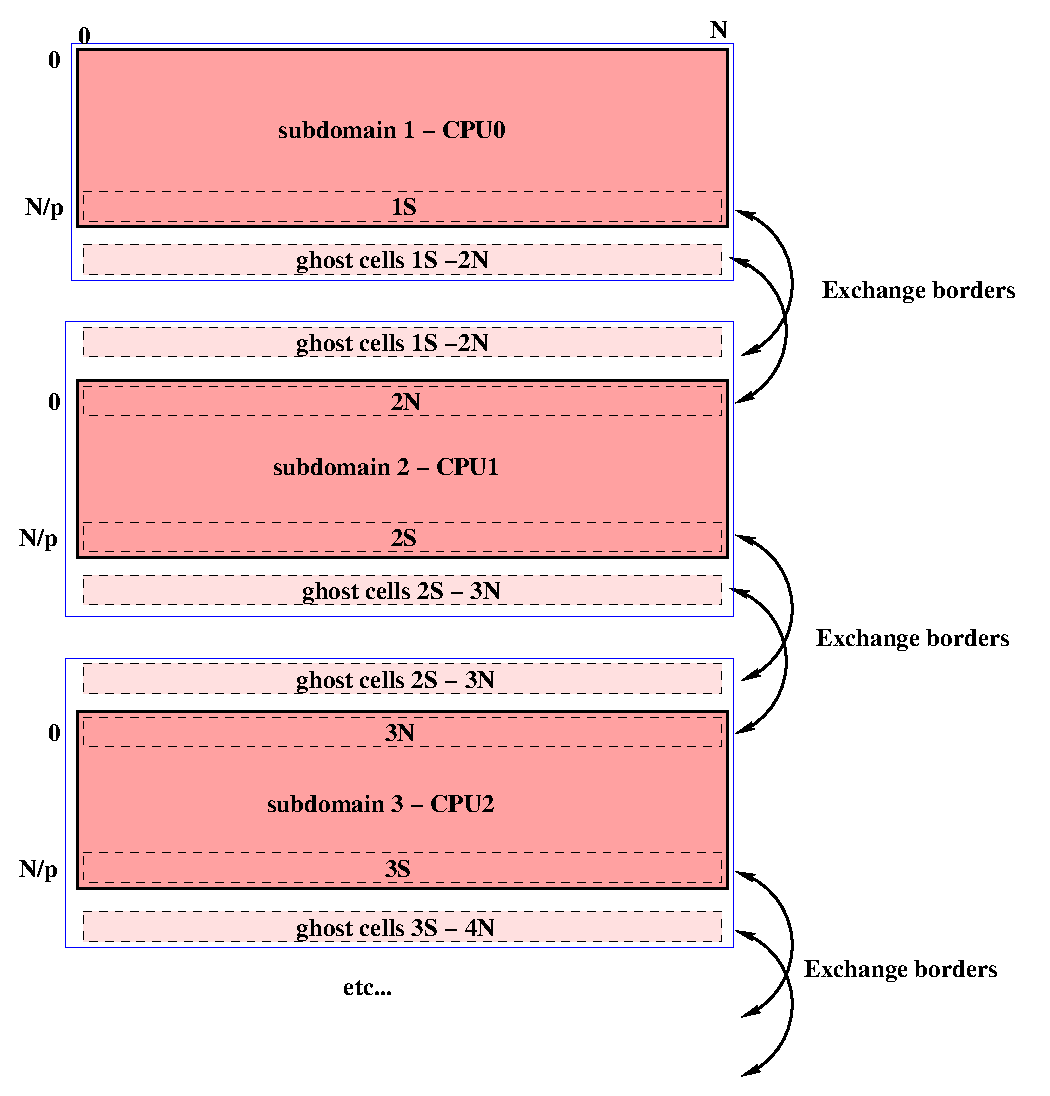
\includegraphics[scale=.6]{images/subdomains.eps}
		\end{center}
		(In Fortran, the memory allocation is ``Column-Major Order'' (make the decomposition by columns))
	}
	\item {Try to keep the size of the MPI messages as large as possible (i.e. send/receive a full line instead of single elements). In order to avoid deadlocks, use $MPI_\_Sendrecv$ first.}
	\item {Same problem as with OpenMP : the main bottleneck is the file writings : remove the call to write$\_$to$\_$file(). The verification is done by comparing the number of iterations to reach a given error ($L2$). To be sure your parallel implementation is correct : compare your results against the serial implementation. }
	\item {To increase the performance of your code, the communications can be hidden behind computation by using non-blocking communications ($MPI\_Isend$)}
\end{itemize}

{\bf Remember : each MPI process runs the same executable !}
\\

\begin{itemize}
	\item{ Increase the size of the grid so that the total execution time on one node is close to 3-4 minutes }
	\item{ Run your application on an increasing number of nodes by fixing the total size of the problem. Draw a log-log graph with the speedup ($S_p = t_1/t_p$) on the y axis, the number of nodes on the x axis (\textbf{strong scaling})}
	\item{ Run your application on an increasing number of nodes by fixing the size of the problem per processor. Draw a graph with the parallel efficiency ($E_p = S_p/p$) on the y axis, the number of nodes on the x axis (\textbf{weak scaling}) }	
\end{itemize}
\end{exercise}
\end{document}
